\documentclass[../../main.tex]{subfiles}

\graphicspath{{\subfix{images/}}}

\begin{document}

\chapter{Componente Disponibile}

\section{Text}

Textul reprezintă componenta de bază a lucrării dumneavoastră.

Deși în majoritatea cazurilor apare în cea mai simplistă versiune posibilă. fără vreo formatare specifică, el poate fi evidențiat prin \textbf{îngroșare}, \textit{înclinare} sau prin \textbfit{ambele metode}.

În interiorul textului, pot fi plasate chiar și scurte secvențe de cod, de e\-xemplu \inlinecode{line.split(":", 1)[0] for line in open("/etc/passwd")}.

De menționat este faptul că împărțirii în silabe a unor cuvinte din limba română nu îi este asigurată corectitudinea. Putem verifica însă textul manual și folosi \textit{tag}-urile \inlinecode{\textbackslash -} pentru a marca unde trebuie efectuată acea împărțire și \inlinecode{\textbackslash mbox} pentru a marca un cuvânt ca fiind monosilabic.

\section{Tabele}

Tabelele sunt aranjări a informației într-o structură formată din linii și coloane, care permite o mai bună observare a acesteia.

Mai jos apar două exemple. Primul tabel este de dimensiune mică. Al doilea, din cauza dimensiunii mai mari, are o orientare inversată și este plasat singur pe o pagină.

\begin{table}[h]
    \begin{tabular}{ | p{0.5\linewidth} | p{0.5\linewidth} | }
        \hline
        Nume Complet & Funcție Ocupată \\
        \hline
        Joshua Roob & Manager de Proiect \\
        Asa Hauck & Artist Grafic \\
        Harley Hagenes & Programator \\
        \hline
    \end{tabular}
    \caption{Colaboratori la Realizarea Studiului}
    \label{tab:small_table}
\end{table}

\newpage

\begin{landscape}
    \vspace*{\fill}
    \begin{table}[h]
    \centering
    \resizebox{19.5cm}{!}{
        \begin{tabular}{ | p{0.25\linewidth} | p{0.25\linewidth} | p{0.25\linewidth} | p{0.25\linewidth} | }
            \hline
            Stat & Oraș & Latitudine & Longitudine \\
            \hline
            South Carolina & Corwinberg & 86.609523 & 42.408007 \\
            Rhode Island & East Isaacmouth & 63.17309 & -13.786023 \\
            Mississippi & North Noblestad & -31.316834 & 5.280483 \\
            Illinois & Grahamland & -39.853659 & -77.713676 \\
            Rhode Island & West Richardfurt & 67.583131 & 31.858455 \\
            Florida & Port Roberta & 25.276026 & 83.715344 \\
            \hline
        \end{tabular}
    }
    \caption{Locații de Conducere a Studiului}
    \label{tab:modules_per_servers}
\end{table}
    \vspace*{\fill}
\end{landscape}

\newpage

\section{Imagini}

Imaginile sunt utilizate în cadrul lucrării pentru exemplificarea unor idei în manieră vizuală.

\begin{center}
    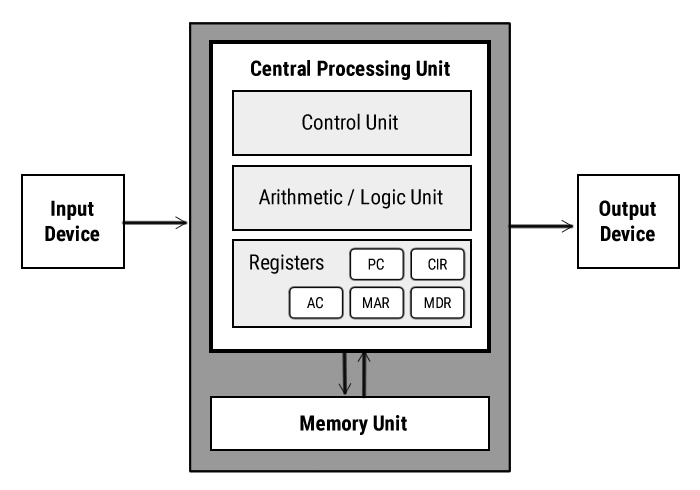
\includegraphics[width=7cm]{components/images/architecture.jpg}
    \label{fig:architecture}
    \captionsetup{justification=centering,margin=1cm}
    \captionof{figure}[Arhitectura unui calculator]{Arhitectura unui calculator\footnotemark}
\end{center}
\vspace{0.3cm}

\footnotetext{Arhitectura ilustrată este de fapt cea von Neumann.}

\section{Liste}

Listele sunt simple serii de informații.

\begin{itemize}
    \item Un item
    \item Unul dintre itemi
    \item Încă un item
\end{itemize}

Acestea pot conțin itemi identificați prin numere dacă indexarea sau sortarea sunt necesare.

\begin{enumerate}
    \item Primul item
    \item Al doilea item
    \item Al treilea item
\end{enumerate}

\section{Formule Matematice}

\LaTeX{} oferă un mod programatic de a construi formule matematice, după cum este cea de mai jos.

\newpage

$ \sum \mathbf{F} = 0 \Leftrightarrow {\frac {\mathrm{d} \mathbf{v}}{\mathrm{d} t}} = 0 $

\section{Note de Subsol. Citări}

Notele de subsol pot fi utile în cazul explicațiilor suplimentare (cum a fost cea referitoare la imaginea inclusă, la care sintaxa este puțin diferită din cauza plasării notei în cadrul legendei) sau a citărilor\footnote{\fullcite{morphological_operations}} care nu se pretează a fi trecute în bibliografie din cauza utilizării lor punctuale.

Pe de altă parte, sursele bibliografice citate intens \cite{cloud_crypto} sunt marcate corespunzător și notate în bibliografie.

\section{Etichete. Referințe}

În cadrul surselor \LaTeX{} a acestui document, apar \textit{tag}-uri \inlinecode{\textbackslash label} care creează o etichetă utilă referințelor interne. Acestea din urmă indică elemente din cadrul documentului curent (de exemplu, către tabelul \ref{tab:small_table}).

Mai pot apărea referințe externe, către resurse din Internet (de exemplu, către \textit{website}-ul \href{https://www.wikipedia.org/}{Wikipedia}).

\end{document}